\chapter{HElib Design} \label{chap:HElibDesign}
\section{HElib Serial Design} \label{sec:HElibSerialDesign}

\begin{figure}[htp]
\centering
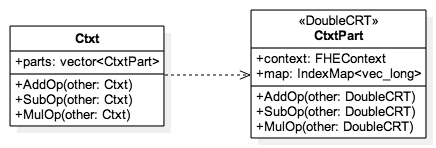
\includegraphics[width=0.65\textwidth]{CtxtTypeHierarchy.png}
\caption{HElib Type Hierarchy}
\label{fig:CtxtTypeHierarchy}
\end{figure}
Before addressing the changes present in the modified libraries, it is necessary to understand the current serial implementation of HElib. Let $\ast$ be the operation being perform (here $\ast$ could stand for any of the operations, all of them are handled similarly) and $A$ and $B$ be the ciphertexts being operated on. The execution of the operation $ A = A\ \ast\  B$ requires a few steps. 

$A$ and $B$ are stored as \verb|Ctxt| objects in HElib. Figure \ref{fig:CtxtTypeHierarchy} shows the type hierarchy for a \verb|Ctxt| object. \verb|Ctxt| objects have one important variable, \verb|parts|, a vector containing multiple \verb|CtxtPart|s. These parts constitute the ciphertext. The operations supported by \verb|Ctxt| are the addition, subtraction, and multiplication of two \verb|Ctxt| objects. Each of these operations use \verb|parts| during the execution of the operation, thus the operations in \verb|CtxtPart| are called.

\verb|CtxtPart| is an extension of the class \verb|DoubleCRT|, which is where the operations are implemented. Listing \ref{lst:HElibSerial} is an excerpt from the function that performs the operations.

\begin{lstlisting}[language=C++,caption={Add, Sub and Mul operations of two DoubleCRT objects},label={lst:HElibSerial}]
...
const IndexSet& s = map.getIndexSet();
long phim = context.zMStar.getPhiM();

for (long i = s.first(); i <= s.last(); i = s.next(i)) {
    long pi = context.ithPrime(i);
    vec_long& row = map[i];
    const vec_long& other_row = (*other_map)[i];

    for (long j = 0; j < phim; j++) {
      row[j] = fun.apply(row[j], other_row[j], pi);
    }
}
...
\end{lstlisting}

As the index set is iterated over, the ith prime is extracted along with the ith row from the maps. Even though the map is accessed like an array, it is an unordered map, with the array access syntax for convenience. These rows are then iterated over, applying the operation to each element. This is where the SIMD design is occurring. A double \verb|for| loop to add, subtract or multiply two vectors together. This is where the modifications can occur.